\chapter{Evaluation}
\label{sec:eval} 

\begin{figure}[H]
    \hspace*{-2.5cm}
    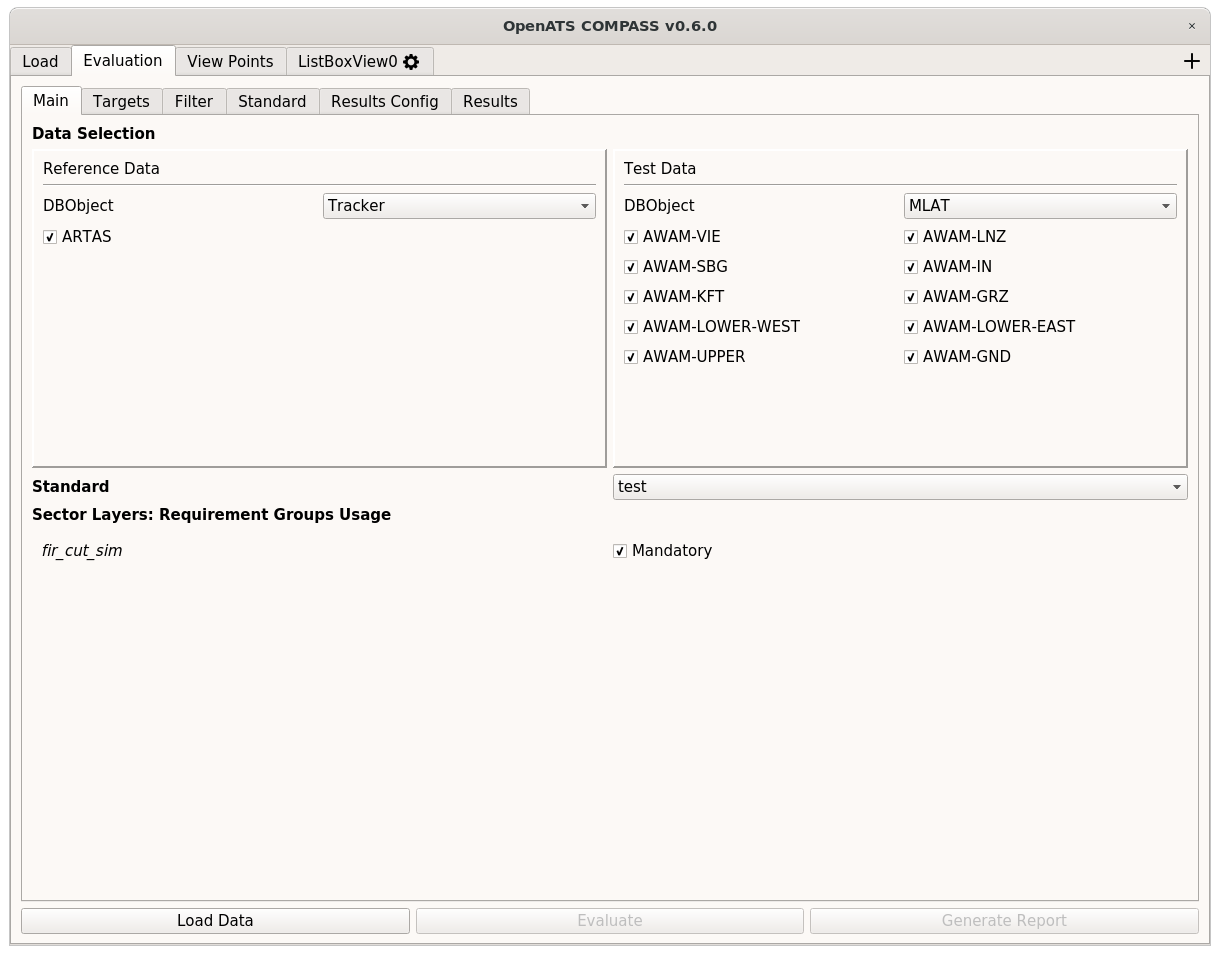
\includegraphics[width=19cm]{../screenshots/evaluation.png}
  \caption{Evaluation tab}
\end{figure}

The 'Evaluation' tab allows adapting/defining requirement-based standards  and compliance assessment of said standards. \\

\section{Pre-Requisites \& Limitations}
\label{sec:eval_prereq} 

\begin{itemize}  
\item Target report associations must be set (using \nameref{sec:task_associate_tr})
\item At least 1 sector has to be defined (using \nameref{sec:task_manage_sectors})
\item Usable reference data must exist
\item Usable test data must exist
\end{itemize}
\ \\

While it is possible to manually remove single targets from the evaluation, the usage of correct reference data is paramount for the significance of the evaluation results. \\

\includegraphics[width=0.5cm]{../../data/icons/hint.png} \textbf{Please note that the evaluation feature is currently severly limited and under heavy development, and should not be used as a sole basis for decision making - especially not without manually verifying the evaluation results.} \\

There will be improvements in the next releases, and further verification of the results by the author and other users.

\subsection{Target Report Associations}

Since the task only makes use of the Mode S address, non-Mode S data is not evaluated and may even show up as gaps/misses in detection.

\subsection{Sector Altitude Filtering}

If sectors with altitude limits are used, please be aware that target reports without a Mode C code can not be filtered by the set limit. Therefore such target reports "show up" in all sectors (as long as inside the defined polygons). \\

The 'inside-sector' is always performed on the reference data only, therefore it is of importance to only use reference data with existing Mode C code data.

\subsection{Reference Data}

The assumption used in the tool is that the reference data is always correct. Therefore, sub-optimal reference data will show up attributed to errors in the test data. \\

To give a few examples what this could mean:
\begin{itemize}  
\item Missing target data in reference: This will remove the test data from evaluation for the time-period of the missing reference data
\item Wrong position in reference: This will cause wrong 'inside sector' check results, and/or cause wrong horizontal position accuracy results
\item Wrong/missing Mode C code in reference: This will cause wrong 'inside sector' check results and might remove the test data from evaluation or associate the results to the wrong sector
\item Wrong/missing identification in reference: This will cause wrong results in identification requirements
\end{itemize}
\ \\

\section{Overview}
\label{sec:eval_overview} 

\begin{figure}[H]
  \hspace*{-2cm}
    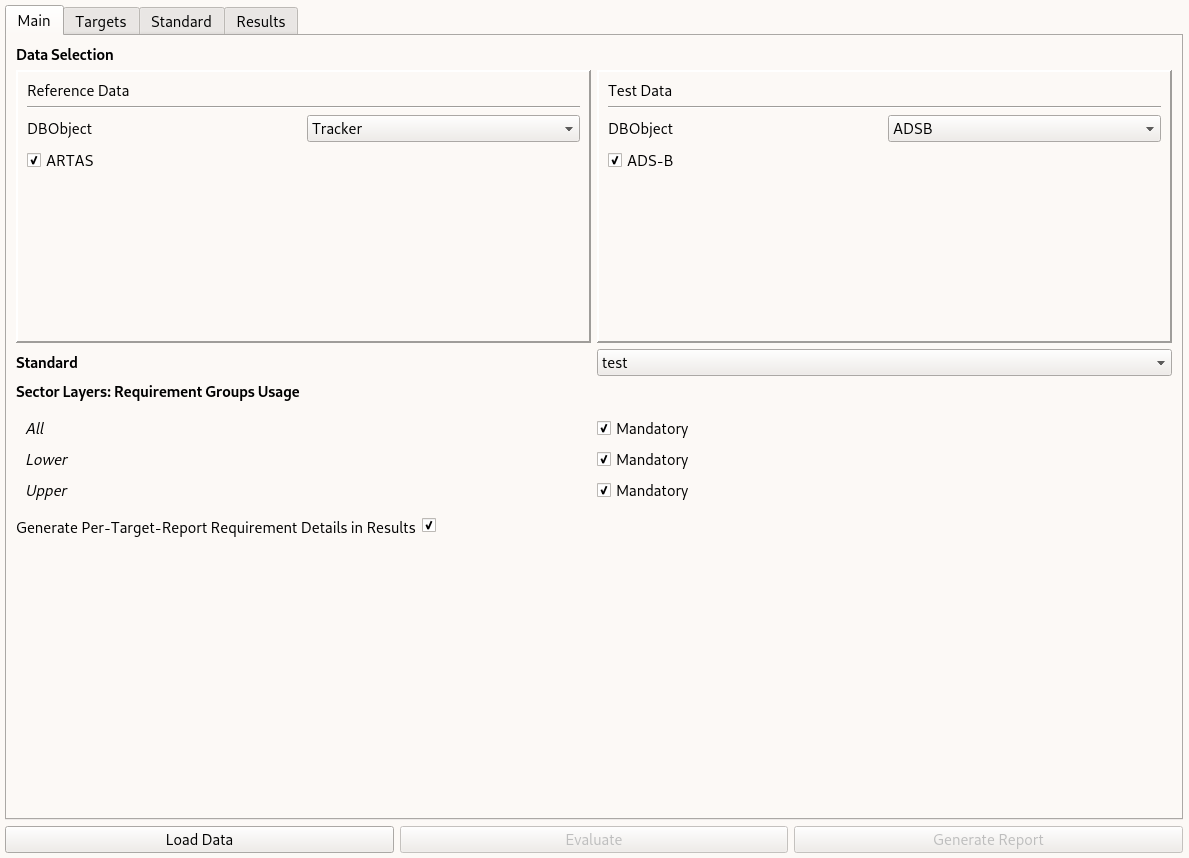
\includegraphics[width=18cm,frame]{../screenshots/eval_overview.png}
  \caption{Evaluation overview}
\end{figure}

At the top, 4 tabs exist:
\begin{itemize}  
\item Main: Main configuration
\item Targets: Table of existing targets (filled after data was loaded)
\item Standard: Definition of standards, selection of current standard, configuration of requirements to be checked
\item Results: Evaluation results (created after data was evaluated)
\end{itemize}
\ \\

Below 3 buttons exist:
\begin{itemize}  
\item Load Data: Loads the reference/test data
\item Evaluate: Runs the evaluation of the current standard (available after data was loaded)
\item Generate Report: Generates a report PDF (available after data was evaluated)
\end{itemize}
\ \\

\section{Configuration}
\label{sec:eval_config} 

\subsection{Main Tab}

\begin{figure}[H]
  \hspace*{-2cm}
    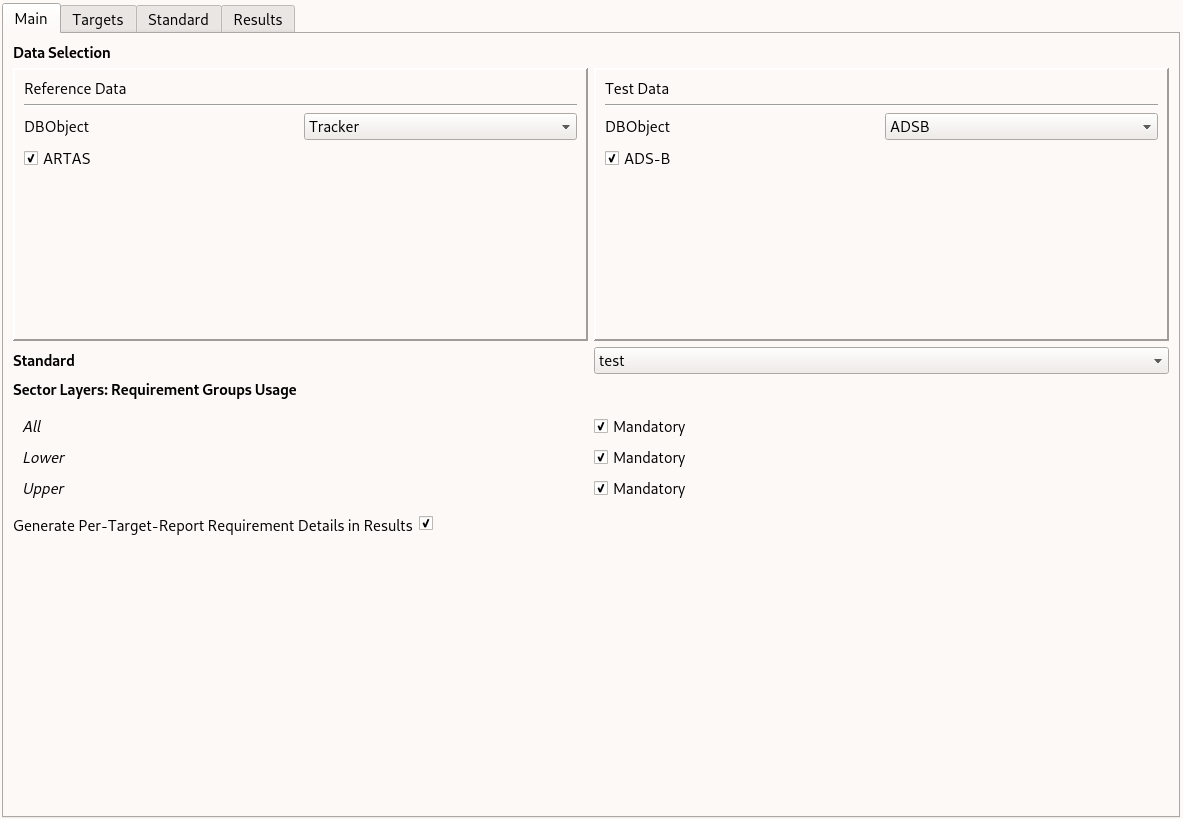
\includegraphics[width=18cm,frame]{../screenshots/eval_main.png}
  \caption{Evaluation Main tab}
\end{figure}

In the main tab, the main configuration settings can be set. \\

\subsubsection{Data Selection}

At the top, the 'Data Selection' can be performed, by selecting:
\begin{itemize}  
\item Reference Data:
\begin{itemize}  
\item DBObject: Any DBObject existing in the database
\item Data source checkboxes: Which data sources to use
\end{itemize}
\item Test Data:
\begin{itemize}  
\item DBObject: Any DBObject existing in the database
\item Data source checkboxes: Which data sources to use
\end{itemize}
\end{itemize}
\ \\

As noted before, usage of appropriate reference data is of paramount importance. \\

Since 'any' type of data can be selected for evaluation, this allows for the following use-cases:
\begin{itemize}  
\item Tracker as reference, Sensor as test data: Evaluation of sensor
\item Tracker as reference, Tracker as test data: Evaluation/comparison of different trackers/tracker runs
\end{itemize}
\ \\

Of course it is also possible to use e.g. an imported GPS trail as reference (see \nameref{sec:task_import_gps}), although this is currently not tested for lack of test data. If you might be able to provide such test data, please contact the author. \\

\subsubsection{Standard}
In the center, using the 'Standard' drop-down menu, the current standard can be selected. To create/configure the standard please use the 'Standard' tab.

\subsubsection{Sector Layer/Requirement Mapping}

Below that, the 'Sector Layers: Requirement Groups Usage' allows to define which requirements should be verified for which sector layer. \\

On the left, all existing sector layers are listed, in the show example:
\begin{itemize}  
\item All: DOI without altitude limitation
\item Lower: Same DOI with altitude limitation, i.e. everything below a certain flight level
\item Upper: Same DOI with altitude limitation, i.e. everything above a certain flight level
\end{itemize}
\ \\

For each sector layer, the requirement groups (defined in the Standard tab) can be active/disabled. In the shown example, the existing requirement group 'Mandatory' is active in all 3 sector layers.

\subsubsection{Other}

The 'Generate Per-Target-Report Requirement Details in Results' checkbox allows to toggle if the per-target-report details should be generated in the evaluation results. \\

If active, this allows for per-target-report inspection of the results, but uses more system memory and makes generation of the report PDF infeasible (10000+ pages). It is recommended to disable generation of these details for large evaluations (e.g. 10+ million target reports, depending on available system memory) or when a report PDF should be generated. \\

Please note that it is possible to first generate the per-target-report details, inspect the results, de-activate the details again, re-run the evaluation and then generate the report PDF.

\subsection{Targets Tab}

\begin{figure}[H]
  \hspace*{-2cm}
    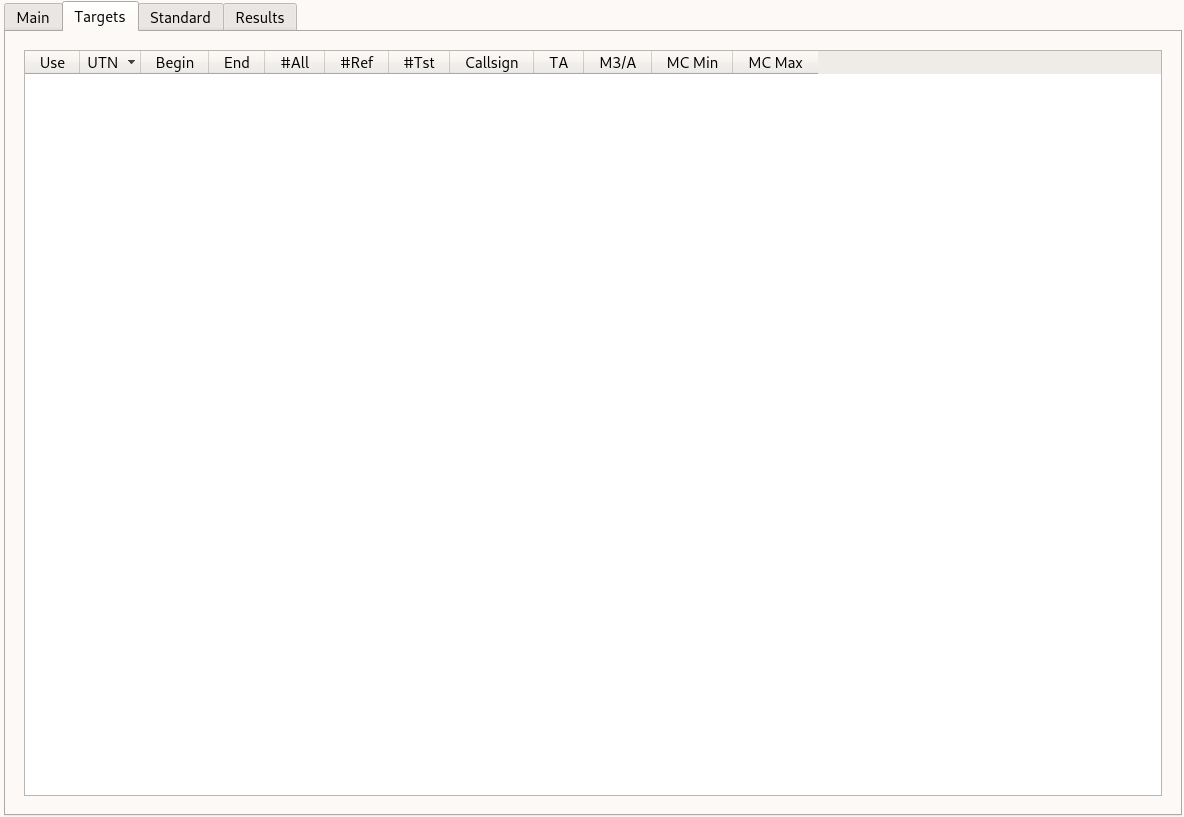
\includegraphics[width=18cm,frame]{../screenshots/eval_targets_empty.png}
  \caption{Evaluation Targets tab}
\end{figure}

Before the data is loaded, the table is empty. Each target (defined by the UTN) is shown in a dedicated row. \\

The following columns exist:

\begin{itemize}  
\item Use: Checkbox defining if the target should be used in the evaluation
\item UTN: Unique Target Number
\item Begin: First timestamp of UTN
\item End: Last timestamp of UTN
\item \#All: Sum number of target reports
\item \#Ref: Number of target reports in reference data
\item \#Tst: Number of target reports in test data
\item Callsign: Target identification(s)
\item TA: Target address (hexadecimal)
\item M3/A: Mode 3/A code(s) (octal)
\item MC Min: Mode C code minimum [ft]
\item MC Max: Mode C code maximum [ft]
\end{itemize}
\ \\

Unless otherwise specified, the column content reflects the values from both reference and test data.

\subsection{Standard Tab}

\begin{figure}[H]
  \hspace*{-2cm}
    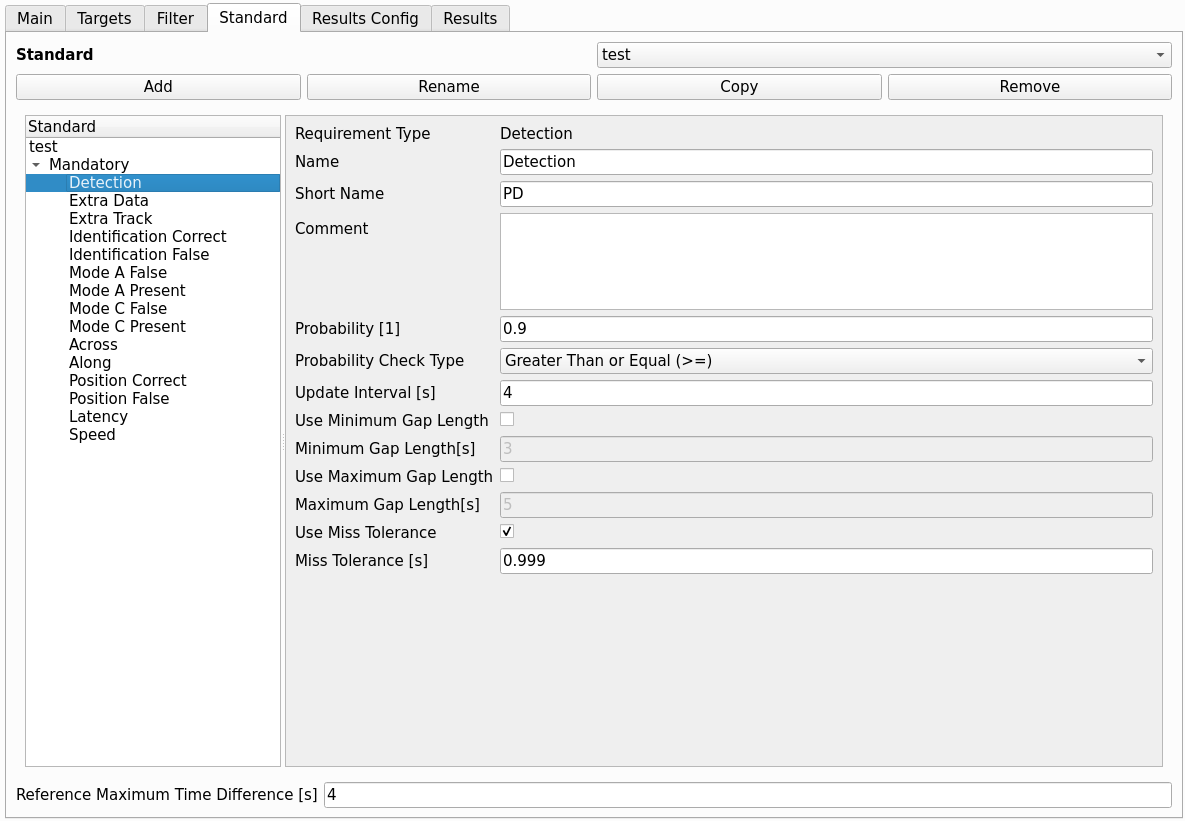
\includegraphics[width=18cm,frame]{../screenshots/eval_standard.png}
  \caption{Evaluation Standard tab}
\end{figure}

In the Standard tab, at the top the current standard can be selected. \\

Below, the following buttons exist:
\begin{itemize}  
\item Add: Add a new standard with a unique name
\item Rename: Rename the current standard (currently disabled)
\item Copy: Copy the current standart to a new one (currently disabled)
\item Remove: Delete current standard
\end{itemize}
\ \\

\subsubsection{Current Standard}

Below that, the current standard is shown. On the left side, a tree-view exists showing:
\begin{itemize}  
\item Standard name
\begin{itemize}  
\item Requirement Group(s)
\begin{itemize}  
\item Requirement(s)
\end{itemize}
\end{itemize}
\end{itemize}
\ \\

When clicking on the standard name, a menu is shown allowing adding new requirement groups ('Add Group'). \\

When clicking on a requirement group, a menu is shown allowing the following functions:
\begin{itemize}  
\item Delete Group: Delete the clicked requirement group
\item Add Requirement:
\begin{itemize}  
\item Detection
\item Identification
\item Position
\end{itemize}
\end{itemize}
\ \\

If a requirement is clicked, it's configuration widget is shown on the right hand side. \\

Each requirement has the following common attributes:
\begin{itemize}  
\item Name: Name of the requirement
\item Short Name: Abbreviated name of the requirement
\end{itemize}
\ \\

\subsubsection{Detection Requirement}

\begin{itemize}  
\item Update Interval [s]: Update interval of the test data
\item Maximum Reference Time Difference [s]: Maximum time delta to closest reference target report
\item Minimum Probability [1]: Minimum probability of detection
\item Use Miss Tolerance: Checkbox if miss tolerance should be used
\item Miss Tolerance [s]: Acceptable time delta for miss detection
\end{itemize}
\ \\

Please note that the exact requirement calculation method is quite complex and will be added at a later point. \\

As a summary, the reference is used to calculate the number of expected update intervals inside the sector layer (EUI). Then, for the test data, if the reference exists at the time, time differences between target reports are checked and the number of misses/gaps are calculated as number of missed update intervals (MUI). \\

The ratio of MUI and EUI gives the probability of missed update interval, the counter-probability gives the Probability of Detection (PD). The PD must be higher than the defined 'Minimum Probability' for the requirement to pass.

\subsubsection{Identification Requirement}

\begin{itemize}  
\item Maximum Reference Time Difference [s]: Maximum time delta to closest reference target report
\item Minimum Probability [1]: Minimum probability of detection
\end{itemize}
\ \\

Please note that the exact requirement calculation method is quite complex and will be added at a later point. \\

As a summary, the reference is used to check each target report's Mode S Target Identification (TI). A TI is incorrect if set in both reference and test data and different, resulting in the number of false TIs (\#FID) and correct TIs (\#CID). \\

The ratio of \#CID and \#FID+\#CID gives the Probability of Correct Identification (PID). The PID must be higher than the defined 'Minimum Probability' for the requirement to pass.

\subsubsection{Position Requirement}

\begin{itemize}  
\item Maximum Reference Time Difference [s]: Maximum time delta to closest reference target report
\item Maximum Distance [m]: Maximum allowed distance from test target report to reference
\item Minimum Probability [1]: Minimum probability of detection
\end{itemize}
\ \\

Please note that the exact requirement calculation method is quite complex and will be added at a later point. \\

As a summary, the reference is used to check each test target report's position. The position is incorrect if the reference position exists and the distance (to the reference position at the same time as the test target report, using linear interpolation) is larger than the defined threshold. This results in the number of incorrect positions (\#PNOK) and correct positions (\#POK). \\

The ratio of \#POK and \#PNOK+\#POK gives the Probability of Acceptable Position (POK). The POK must be higher than the defined 'Minimum Probability' for the requirement to pass.

\subsection{Results Tab}

\begin{figure}[H]
  \hspace*{-2cm}
    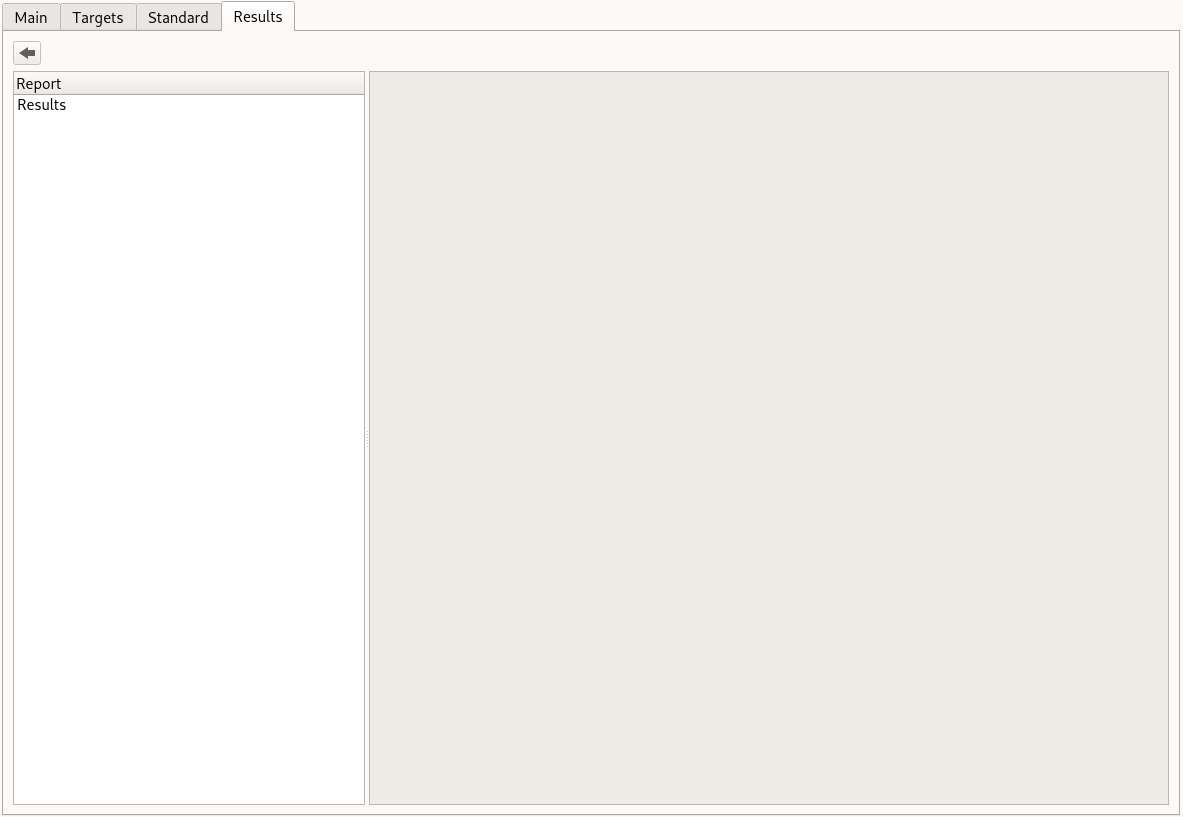
\includegraphics[width=18cm,frame]{../screenshots/eval_results_empty.png}
  \caption{Evaluation Results tab}
\end{figure}


\section{Running}
\label{sec:eval_run} 

loading

\begin{figure}[H]
  \centering 
    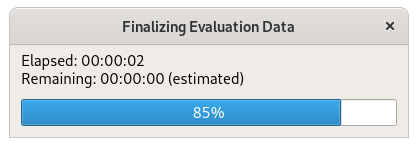
\includegraphics[width=8cm]{../screenshots/eval_post.png}
  \caption{Evaluation: Post-processing after loading}
\end{figure}

\begin{figure}[H]
  \hspace*{-2cm}
    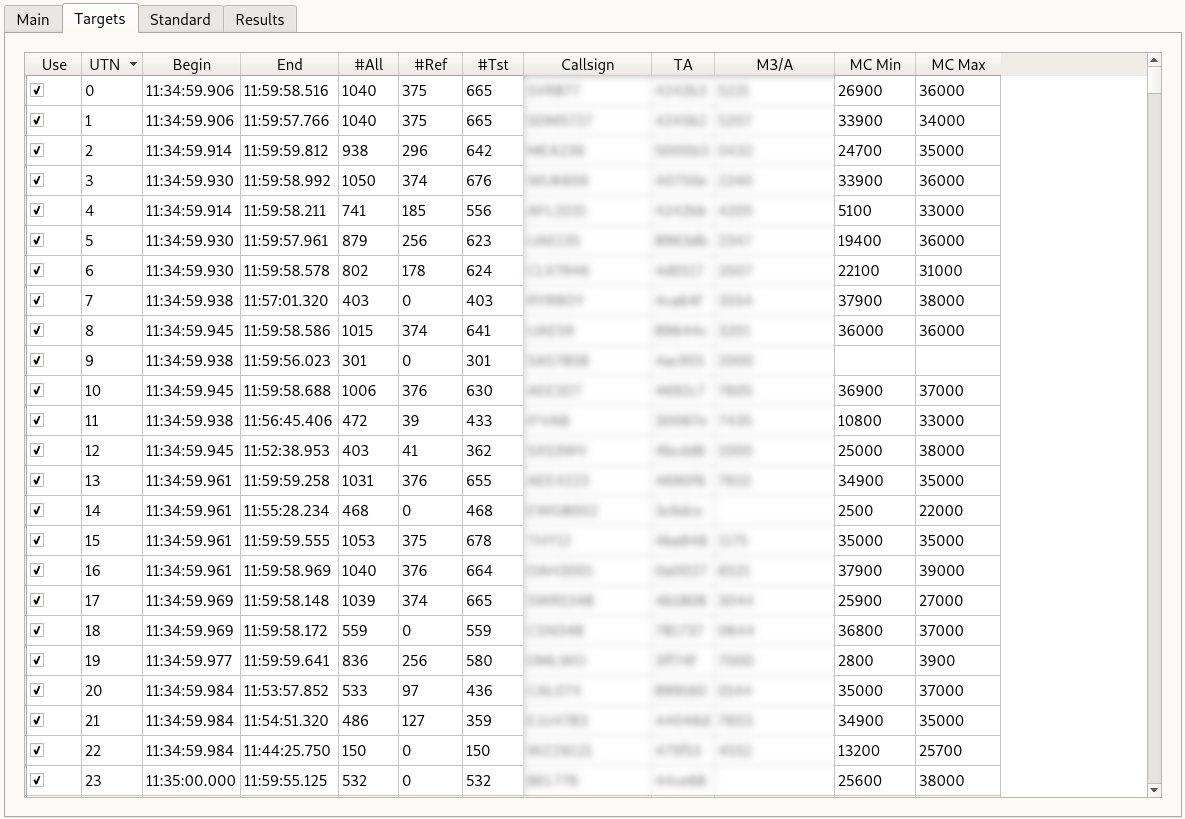
\includegraphics[width=18cm,frame]{../screenshots/eval_targets.png}
  \caption{Evaluation Targets tab after loading}
\end{figure}

eval

\begin{figure}[H]
  \centering 
    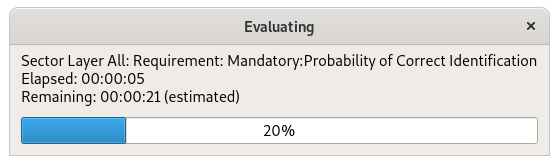
\includegraphics[width=10cm]{../screenshots/eval_eval_status.png}
  \caption{Evaluation: Running evaluation status}
\end{figure}

\section{Inspection \& Analysis}
\label{sec:eval_inspect} 

\section{Generate Report}
\label{sec:eval_report}
